\section{基于图序列生成标定结果}\label{sec:4}

在上述流程中,我们对视频数据中的每一帧生成了一张对应的蒙版。该蒙版记录了钡餐区域的本底值数据。现在我们来到了最后一部分,即基于这些本底值数据得到最终的钡餐区域和浓度标定结果。

\subsection{定义}\label{sec:4_1}
\begin{itemize}
    \item 我们将一组(经过预处理后的)医学视频数据记为 $D$。其中第 $k$ 帧所代表的二维灰度图像为 $D[k]$。该图像中像素 $[x, y]$ 处的灰度值为 $D[k, x, y]$。
    \item 我们将通过 $D[k]$ 所求得的视频第 $k$ 帧对应的钡餐区域及其本底值记为 $T[k]$。对于 $T[k]$ 中的像素 $[x, y]$,记 $T[k, x, y]=t$。若 $t=0$,代表该像素在该帧中非钡餐区域;反之,代表该像素在该帧属于钡餐区域,且算法认为该像素点在成为钡餐区域之前,其所对应的人体器官或组织的像素值为t。在最终逐帧逐像素标记钡餐浓度时,应根据此本底值做出修正。
    \item 对于数组 $T$,维护一个与之一一对应的布尔数组 $F$。若 $F[i]$ 为真,代表尝试使用 $T[i]$ 进行扩张,反之不使用。
    \item 我们将最终的钡餐区域及浓度标定结果数据记为 $R$。对于第 $k$ 帧中的像素 $[x, y]$,记 $R[k, x, y]=r$。若 $r=0$,代表该像素在该帧中非钡餐区域;反之,代表该像素在该帧中属于钡餐区域,且其相对浓度为 $r$。$r$ 的取值范围为 $[0, 255]$,数值越大代表其相对浓度越高。
\end{itemize}

\subsection{方法描述}

事实上,在上述流程中,每一帧求得的钡餐本底值蒙版不一定能完整地标注出钡餐区域。由于该蒙版是通过绝对差图像处理得到的,因此当且仅当某一帧中整个钡餐区域的边界相较上一帧在各个方向都有的运动时,蒙版中的钡餐区域才具有较高的准确度。在实际数据中,受试者将钡餐含在口中不咀嚼时,钡餐的运动可能较为平缓;而受试者在吞咽钡餐时,钡餐沿着喉管运动,其方向沿着呈现强烈的指向性。在这些情景下,绝对差图像中无法表现出完整的轮廓,进而导致钡餐区域标注不准确。在\cref{fig:4_示意图} 中,我们用一组简化的图像说明该情况。

\begin{figure}[!htp]
    \centering
    \begin{subfigure}{\textwidth}
        \centering
        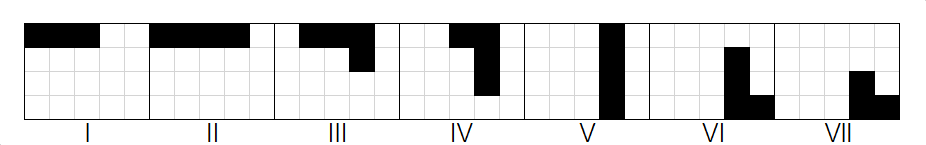
\includegraphics[width=0.8\textwidth]{figures/4_示例_1.png}
        \caption{原始数据}
    \end{subfigure}
    \begin{subfigure}{\textwidth}
        \centering
        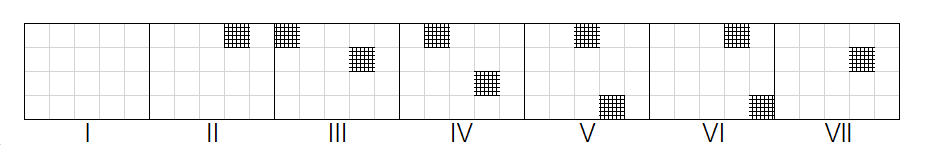
\includegraphics[width=0.8\textwidth]{figures/4_示例_2.png}
        \caption{运动区域}
    \end{subfigure}
    \begin{subfigure}{\textwidth}
        \centering
        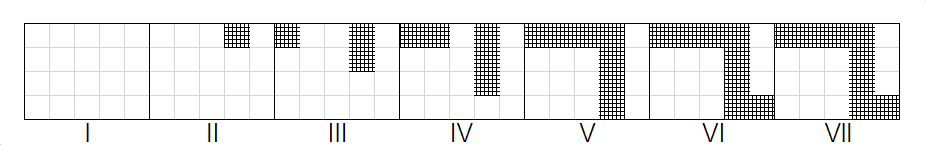
\includegraphics[width=0.8\textwidth]{figures/4_示例_3.png}
        \caption{运动区域叠加}
    \end{subfigure}
    \begin{subfigure}{\textwidth}
        \centering
        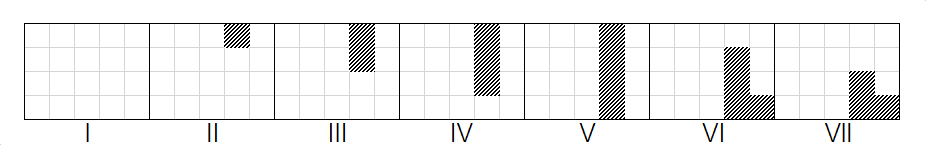
\includegraphics[width=0.8\textwidth]{figures/4_示例_4.png}
        \caption{运动区域叠加后与原始数据求交}
    \end{subfigure}
    \caption{简化示意图}
    \label{fig:4_示意图}
\end{figure}

在\cref{fig:4_示意图}(a) 中,我们展示了一组钡餐的运动过程,共7帧。每一帧中的黑色的部分代表钡餐。在图中,钡餐首先被拉伸,随后向下移动至底部拐弯,最后收缩。\cref{fig:4_示意图}(b) 展示了原始数据的绝对差图像,其中方格部分代表该帧与前一帧不同之处,即钡餐的运动部分。观察可知,在该样例下,通过绝对差图像最终得到的蒙版无法与实际钡餐区域准确对应。

为解决此问题,需充分利用连续时间段内所有图像的信息,而非仅关注相邻帧间的差异。我们可以注意到以下结论:除第一帧中钡餐所在的区域,若某坐标在某帧属于钡餐区域,则该坐标必然在此帧或其前驱帧中从非钡餐区域转变为钡餐区域。如果我们将\cref{fig:4_示意图}(b) 中的每帧与其所有前驱帧叠加,可得到\cref{fig:4_示意图}(c),每帧图像表示截至当前帧,所发现的所有当前或曾经属于钡餐的区域。\cref{fig:4_示意图}(d) 展示了将 (c) 图与 (a) 图取交集的结果。如此一来,除初始几帧外,(d) 中的后续帧与原始数据吻合。这说明(c) 中(除初始几帧外)的图像可以在将原始数据的大部分区域过滤的同时,保留足够多的感兴趣区域,不遗漏。

在实际数据中,两个帧本底值蒙版之间的操作并不能单纯用“叠加”来概括。因为蒙版并非一个二值图,而是灰度图。我们需要设计相应的方法来处理。此外,在实际操作过程中,我们并不能直接将每一帧与其所有前驱帧叠加,再执行所谓的“求交”操作。因为钡餐区域正是需要我们寻找的目标,而非预先已知的数据。即意味着,我们需要构建某种方法以判断和记录每个帧蒙版的有效性,需要决定每一帧使用哪些前驱帧进行扩展,需要判断何时终止扩展以达到最佳效果。何况,在处理每一帧时,叠加所有前驱帧结果本身便会导致性能问题。

\subsection{操作流程}

在本研究中,对于本底值蒙版数组 $T$,我们维护一个与之一一对应的布尔数组 $F$。若 $F[i]$ 为真,代表尝试使用 $T[i]$ 进行扩张,反之不使用。我们将当前最前驱的有效帧记为 $e$,即:$F[0]=F[1]=...=F[e-1]=\text{False}, F[e]=\text{True}$。

对于第 $i$ 帧,求取 $R[i]$ 的具体步骤如下:
\begin{itemize}
    \item 将 $T[i]$ 的数据拷贝给 $R[i]$。
    \item 对 $i-1$ 到 $e$ 中的每一帧 $k$:
    \subitem 若 $F[k]$ 为真,则使用 $T[k]$ 对 $R[i]$ 进行\textit{扩张}。
    \subitem 若 $T[k]$ 未能更新 $R[i]$ 中的任何一个像素点,则 $F[k]$ 置为假,后续不再考虑第 $k$ 帧。
    \item 更新 $e$ 的值。
    \item $R[i] = R[i] - D[i]$
\end{itemize}

其中,扩张过程遵循以下约定:若第 $k$ 帧中的坐标 $[x, y]$ 的本底值 $T[k, x, y]$ 大于该坐标在第 $i$ 帧的数据值 $D[i, x, y]$,且同时大于 $R[i, x, y]$,则将 $T[k, x, y]$ 赋值给 $R[i, x, y]$。

扩张过程的伪语言描述如下:
\begin{algorithm}
    \caption{扩张过程}\label{algo:expansion}
    \begin{algorithmic}[1]
        \Require 当前帧图像 $d$, 当前帧标定结果 $r$, 待使用的蒙版 $t$
        \Ensure 更新后的帧标定结果 $r$, $r$ 中被蒙版 $t$ 更新的像素数量 $p$
        \Function{ExpandArea}{$d, r, t$}
            \State $x, y \gets d.shape$ % x, y = d.shape
            \State $p \gets 0$ % p = 0
            \For{$i \in \{0, \cdots, x-1\}$} % for i in range(x):
                \For{$j \in \{0, \cdots, y-1\}$} % for j in range(y):
                    \If{$t[i][j] \geq d[i][j]$} % if t[i][j] >= d[i][j]:
                        \If{$t[i][j] > r[i][j]$} % if t[i][j] > r[i][j]:
                            \State $p \gets p + 1$ % p += 1
                            \State $r[i][j] \gets t[i][j]$ % r[i][j] = t[i][j]
                        \EndIf
                    \EndIf
                \EndFor
            \EndFor
            \State \Return $p$ % return p
        \EndFunction
    \end{algorithmic}
\end{algorithm}

\subsection{结果}

由于原始采集仪器数据及环境数据暂缺,无法确定钡餐的绝对浓度,因此以下结果中,浓度标定均采用相对浓度。\cref{fig:4_结果} 展示了两组经过上述操作后得到的钡餐区域和浓度标注。这两组数据中,钡餐分别位于受试者的口部和喉部。每组数据中,从左到右分别为:原始数据帧,由相邻帧得到的钡餐区域及蒙版,使用本章方法扩展得到的钡餐区域及浓度标定。
其中,黑色部分代表非钡餐区域;非黑色部分其亮度越高,代表其相对浓度越高。
\clearpage
\begin{figure}[!htp]
    \centering
    \begin{subfigure}{\textwidth}
        \centering
        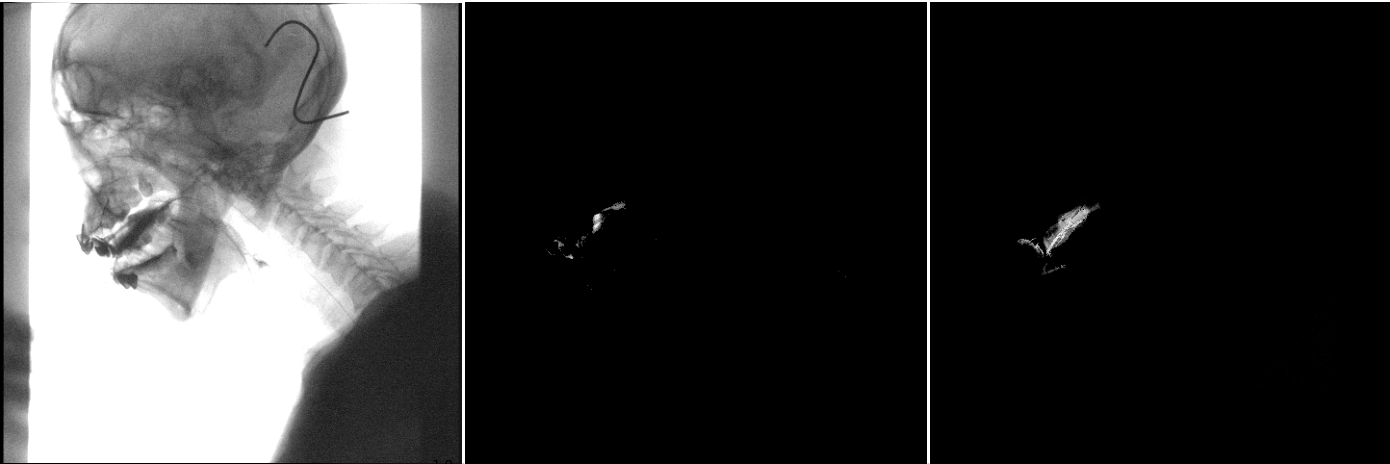
\includegraphics[width=0.9\textwidth]{figures/421.png}
        \caption{口部}
    \end{subfigure}
    
    \begin{subfigure}{\textwidth}
        \centering
        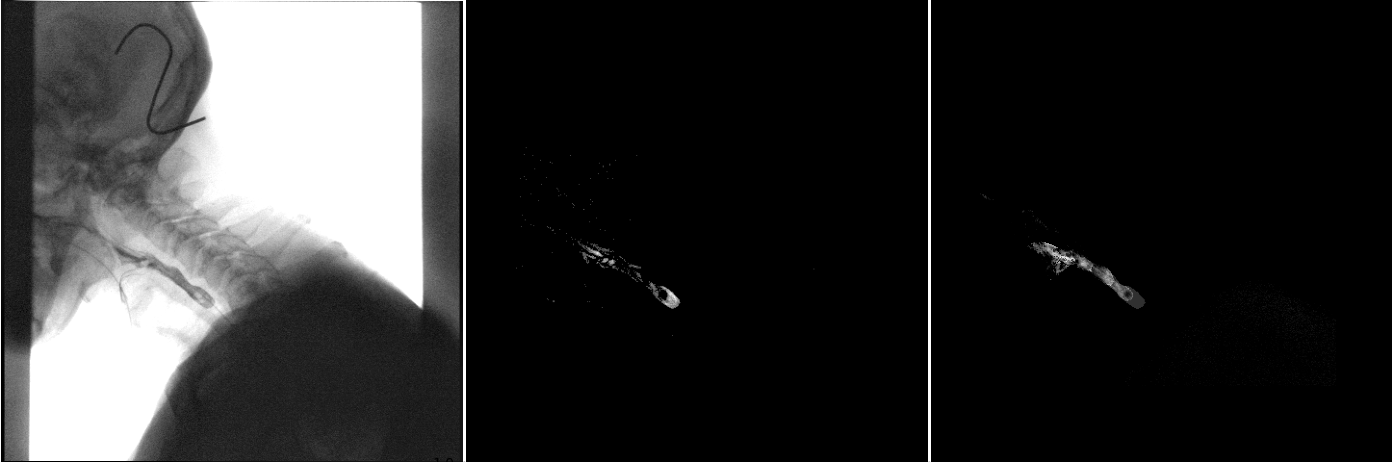
\includegraphics[width=0.9\textwidth]{figures/422.png}
        \caption{喉部}
    \end{subfigure}
    \caption{钡餐区域和相对浓度标注}
    \label{fig:4_结果}
\end{figure}

\subsection{本章小结}

本章中,我们提出一种拓展逐帧操作成果的算法。针对每一帧图像,以上述获得的蒙版作为基础,借助前驱帧所得蒙版进行扩张操作;在此过程中,不断维护各蒙版的有效性,以提高处理速度。最终,我们得到每一帧中的钡餐区域及相对浓度标定。